\documentclass[journal]{IEEEtran}

%============================================================
% PERSONAL LIBRARIES
%============================================================

% For highlighting
\usepackage{soul}

% For degree symbol mainly
\usepackage{siunitx}

\sisetup{
  parse-numbers=false,
  }

% For code blocks
\usepackage{listings}

\usepackage{color}

\definecolor{mygreen}{rgb}{0,0.6,0}
\definecolor{mygray}{rgb}{0.5,0.5,0.5}
\definecolor{mymauve}{rgb}{0.58,0,0.82}

\lstset{ %
  basicstyle=\footnotesize,
  captionpos=b,                    
  commentstyle=\color{mygreen},    
  frame=single,                    
  keywordstyle=\color{blue},       
  language=C++,
  numbers=left,
  numbersep=10pt,
  numberstyle=\tiny\color{mygray},
  stringstyle=\color{mymauve},
  tabsize=2,
  xleftmargin=2em,
  framexleftmargin=2em
}

%============================================================
% LIBRARIES
%============================================================

% Some very useful LaTeX packages include:

% *** MISC UTILITY PACKAGES ***
%
\usepackage{cite}
% cite.sty was written by Donald Arseneau
% V1.6 and later of IEEEtran pre-defines the format of the cite.sty package
% \cite{} output to follow that of IEEE. Loading the cite package will
% result in citation numbers being automatically sorted and properly
% "compressed/ranged". e.g., [1], [9], [2], [7], [5], [6] without using
% cite.sty will become [1], [2], [5]--[7], [9] using cite.sty. cite.sty's
% \cite will automatically add leading space, if needed. Use cite.sty's
% noadjust option (cite.sty V3.8 and later) if you want to turn this off.
% cite.sty is already installed on most LaTeX systems. Be sure and use
% version 4.0 (2003-05-27) and later if using hyperref.sty. cite.sty does
% not currently provide for hyperlinked citations.
% The latest version can be obtained at:
% http://www.ctan.org/tex-archive/macros/latex/contrib/cite/
% The documentation is contained in the cite.sty file itself.





% *** GRAPHICS RELATED PACKAGES ***
%
\usepackage[pdftex]{graphicx}
% declare the path(s) where your graphic files are
% \graphicspath{{../pdf/}{../jpeg/}}
% and their extensions so you won't have to specify these with
% every instance of \includegraphics
% \DeclareGraphicsExtensions{.pdf,.jpeg,.png}

% graphicx was written by David Carlisle and Sebastian Rahtz. It is
% required if you want graphics, photos, etc. graphicx.sty is already
% installed on most LaTeX systems. The latest version and documentation can
% be obtained at: 
% http://www.ctan.org/tex-archive/macros/latex/required/graphics/
% Another good source of documentation is "Using Imported Graphics in
% LaTeX2e" by Keith Reckdahl which can be found as epslatex.ps or
% epslatex.pdf at: http://www.ctan.org/tex-archive/info/
%
% latex, and pdflatex in dvi mode, support graphics in encapsulated
% postscript (.eps) format. pdflatex in pdf mode supports graphics
% in .pdf, .jpeg, .png and .mps (metapost) formats. Users should ensure
% that all non-photo figures use a vector format (.eps, .pdf, .mps) and
% not a bitmapped formats (.jpeg, .png). IEEE frowns on bitmapped formats
% which can result in "jaggedy"/blurry rendering of lines and letters as
% well as large increases in file sizes.
%
% You can find documentation about the pdfTeX application at:
% http://www.tug.org/applications/pdftex





% *** MATH PACKAGES ***
%
\usepackage[cmex10]{amsmath}
% A popular package from the American Mathematical Society that provides
% many useful and powerful commands for dealing with mathematics. If using
% it, be sure to load this package with the cmex10 option to ensure that
% only type 1 fonts will utilized at all point sizes. Without this option,
% it is possible that some math symbols, particularly those within
% footnotes, will be rendered in bitmap form which will result in a
% document that can not be IEEE Xplore compliant!
%
% Also, note that the amsmath package sets \interdisplaylinepenalty to 10000
% thus preventing page breaks from occurring within multiline equations. Use:
%\interdisplaylinepenalty=2500
% after loading amsmath to restore such page breaks as IEEEtran.cls normally
% does. amsmath.sty is already installed on most LaTeX systems. The latest
% version and documentation can be obtained at:
% http://www.ctan.org/tex-archive/macros/latex/required/amslatex/math/





% *** SPECIALIZED LIST PACKAGES ***
%
%\usepackage{algorithmic}
% algorithmic.sty was written by Peter Williams and Rogerio Brito.
% This package provides an algorithmic environment fo describing algorithms.
% You can use the algorithmic environment in-text or within a figure
% environment to provide for a floating algorithm. Do NOT use the algorithm
% floating environment provided by algorithm.sty (by the same authors) or
% algorithm2e.sty (by Christophe Fiorio) as IEEE does not use dedicated
% algorithm float types and packages that provide these will not provide
% correct IEEE style captions. The latest version and documentation of
% algorithmic.sty can be obtained at:
% http://www.ctan.org/tex-archive/macros/latex/contrib/algorithms/
% There is also a support site at:
% http://algorithms.berlios.de/index.html
% Also of interest may be the (relatively newer and more customizable)
% algorithmicx.sty package by Szasz Janos:
% http://www.ctan.org/tex-archive/macros/latex/contrib/algorithmicx/




% *** ALIGNMENT PACKAGES ***
%
%\usepackage{array}
% Frank Mittelbach's and David Carlisle's array.sty patches and improves
% the standard LaTeX2e array and tabular environments to provide better
% appearance and additional user controls. As the default LaTeX2e table
% generation code is lacking to the point of almost being broken with
% respect to the quality of the end results, all users are strongly
% advised to use an enhanced (at the very least that provided by array.sty)
% set of table tools. array.sty is already installed on most systems. The
% latest version and documentation can be obtained at:
% http://www.ctan.org/tex-archive/macros/latex/required/tools/


%\usepackage{mdwmath}
%\usepackage{mdwtab}
% Also highly recommended is Mark Wooding's extremely powerful MDW tools,
% especially mdwmath.sty and mdwtab.sty which are used to format equations
% and tables, respectively. The MDWtools set is already installed on most
% LaTeX systems. The lastest version and documentation is available at:
% http://www.ctan.org/tex-archive/macros/latex/contrib/mdwtools/


% IEEEtran contains the IEEEeqnarray family of commands that can be used to
% generate multiline equations as well as matrices, tables, etc., of high
% quality.


%\usepackage{eqparbox}
% Also of notable interest is Scott Pakin's eqparbox package for creating
% (automatically sized) equal width boxes - aka "natural width parboxes".
% Available at:
% http://www.ctan.org/tex-archive/macros/latex/contrib/eqparbox/


% *** SUBFIGURE PACKAGES ***
%\usepackage[tight,footnotesize]{subfigure}
% subfigure.sty was written by Steven Douglas Cochran. This package makes it
% easy to put subfigures in your figures. e.g., "Figure 1a and 1b". For IEEE
% work, it is a good idea to load it with the tight package option to reduce
% the amount of white space around the subfigures. subfigure.sty is already
% installed on most LaTeX systems. The latest version and documentation can
% be obtained at:
% http://www.ctan.org/tex-archive/obsolete/macros/latex/contrib/subfigure/
% subfigure.sty has been superceeded by subfig.sty.



%\usepackage[caption=false]{caption}
%\usepackage[font=footnotesize]{subfig}
% subfig.sty, also written by Steven Douglas Cochran, is the modern
% replacement for subfigure.sty. However, subfig.sty requires and
% automatically loads Axel Sommerfeldt's caption.sty which will override
% IEEEtran.cls handling of captions and this will result in nonIEEE style
% figure/table captions. To prevent this problem, be sure and preload
% caption.sty with its "caption=false" package option. This is will preserve
% IEEEtran.cls handing of captions. Version 1.3 (2005/06/28) and later 
% (recommended due to many improvements over 1.2) of subfig.sty supports
% the caption=false option directly:
%\usepackage[caption=false,font=footnotesize]{subfig}
%
% The latest version and documentation can be obtained at:
% http://www.ctan.org/tex-archive/macros/latex/contrib/subfig/
% The latest version and documentation of caption.sty can be obtained at:
% http://www.ctan.org/tex-archive/macros/latex/contrib/caption/




% *** FLOAT PACKAGES ***
%
%\usepackage{fixltx2e}
% fixltx2e, the successor to the earlier fix2col.sty, was written by
% Frank Mittelbach and David Carlisle. This package corrects a few problems
% in the LaTeX2e kernel, the most notable of which is that in current
% LaTeX2e releases, the ordering of single and double column floats is not
% guaranteed to be preserved. Thus, an unpatched LaTeX2e can allow a
% single column figure to be placed prior to an earlier double column
% figure. The latest version and documentation can be found at:
% http://www.ctan.org/tex-archive/macros/latex/base/



%\usepackage{stfloats}
% stfloats.sty was written by Sigitas Tolusis. This package gives LaTeX2e
% the ability to do double column floats at the bottom of the page as well
% as the top. (e.g., "\begin{figure*}[!b]" is not normally possible in
% LaTeX2e). It also provides a command:
%\fnbelowfloat
% to enable the placement of footnotes below bottom floats (the standard
% LaTeX2e kernel puts them above bottom floats). This is an invasive package
% which rewrites many portions of the LaTeX2e float routines. It may not work
% with other packages that modify the LaTeX2e float routines. The latest
% version and documentation can be obtained at:
% http://www.ctan.org/tex-archive/macros/latex/contrib/sttools/
% Documentation is contained in the stfloats.sty comments as well as in the
% presfull.pdf file. Do not use the stfloats baselinefloat ability as IEEE
% does not allow \baselineskip to stretch. Authors submitting work to the
% IEEE should note that IEEE rarely uses double column equations and
% that authors should try to avoid such use. Do not be tempted to use the
% cuted.sty or midfloat.sty packages (also by Sigitas Tolusis) as IEEE does
% not format its papers in such ways.


%\ifCLASSOPTIONcaptionsoff
%  \usepackage[nomarkers]{endfloat}
% \let\MYoriglatexcaption\caption
% \renewcommand{\caption}[2][\relax]{\MYoriglatexcaption[#2]{#2}}
%\fi
% endfloat.sty was written by James Darrell McCauley and Jeff Goldberg.
% This package may be useful when used in conjunction with IEEEtran.cls'
% captionsoff option. Some IEEE journals/societies require that submissions
% have lists of figures/tables at the end of the paper and that
% figures/tables without any captions are placed on a page by themselves at
% the end of the document. If needed, the draftcls IEEEtran class option or
% \CLASSINPUTbaselinestretch interface can be used to increase the line
% spacing as well. Be sure and use the nomarkers option of endfloat to
% prevent endfloat from "marking" where the figures would have been placed
% in the text. The two hack lines of code above are a slight modification of
% that suggested by in the endfloat docs (section 8.3.1) to ensure that
% the full captions always appear in the list of figures/tables - even if
% the user used the short optional argument of \caption[]{}.
% IEEE papers do not typically make use of \caption[]'s optional argument,
% so this should not be an issue. A similar trick can be used to disable
% captions of packages such as subfig.sty that lack options to turn off
% the subcaptions:
% For subfig.sty:
% \let\MYorigsubfloat\subfloat
% \renewcommand{\subfloat}[2][\relax]{\MYorigsubfloat[]{#2}}
% For subfigure.sty:
% \let\MYorigsubfigure\subfigure
% \renewcommand{\subfigure}[2][\relax]{\MYorigsubfigure[]{#2}}
% However, the above trick will not work if both optional arguments of
% the \subfloat/subfig command are used. Furthermore, there needs to be a
% description of each subfigure *somewhere* and endfloat does not add
% subfigure captions to its list of figures. Thus, the best approach is to
% avoid the use of subfigure captions (many IEEE journals avoid them anyway)
% and instead reference/explain all the subfigures within the main caption.
% The latest version of endfloat.sty and its documentation can obtained at:
% http://www.ctan.org/tex-archive/macros/latex/contrib/endfloat/
%
% The IEEEtran \ifCLASSOPTIONcaptionsoff conditional can also be used
% later in the document, say, to conditionally put the References on a 
% page by themselves.





% *** PDF, URL AND HYPERLINK PACKAGES ***
%
\usepackage{url}
% url.sty was written by Donald Arseneau. It provides better support for
% handling and breaking URLs. url.sty is already installed on most LaTeX
% systems. The latest version can be obtained at:
% http://www.ctan.org/tex-archive/macros/latex/contrib/misc/
% Read the url.sty source comments for usage information. Basically,
% \url{my_url_here}.


\usepackage{color}

%============================================================
% PRE-DOCUMENT SETUP
%============================================================

% *** Do not adjust lengths that control margins, column widths, etc. ***
% *** Do not use packages that alter fonts (such as pslatex).         ***
% There should be no need to do such things with IEEEtran.cls V1.6 and later.
% (Unless specifically asked to do so by the journal or conference you plan
% to submit to, of course. )


% correct bad hyphenation here
\hyphenation{op-tical net-works semi-conduc-tor}

\begin{document}

%============================================================
% DOCUMENT SETUP
%============================================================

%
% paper title
% can use linebreaks \\ within to get better formatting as desired
\title{Nerf Firing Final Report}
%
%
% author names and IEEE memberships
% note positions of commas and nonbreaking spaces ( ~ ) LaTeX will not break
% a structure at a ~ so this keeps an author's name from being broken across
% two lines.
% use \thanks{} to gain access to the first footnote area
% a separate \thanks must be used for each paragraph as LaTeX2e's \thanks
% was not built to handle multiple paragraphs
%

\author{Craig~Hiller,
Kevin~Wu,
        Leo~Kam, Christopher~Hsu}% <-this % stops a space

% note the % following the last \IEEEmembership and also \thanks -
% these prevent an unwanted space from occurring between the last author name
% and the end of the author line. i.e., if you had this:
% 
% \author{....lastname \thanks{...} \thanks{...} }
%                     ^------------^------------^----Do not want these spaces!
%
% a space would be appended to the last name and could cause every name on that
% line to be shifted left slightly. This is one of those "LaTeX things". For
% instance, "\textbf{A} \textbf{B}" will typeset as "A B" not "AB". To get
% "AB" then you have to do: "\textbf{A}\textbf{B}"
% \thanks is no different in this regard, so shield the last } of each \thanks
% that ends a line with a % and do not let a space in before the next \thanks.
% Spaces after \IEEEmembership other than the last one are OK (and needed) as
% you are supposed to have spaces between the names. For what it is worth,
% this is a minor point as most people would not even notice if the said evil
% space somehow managed to creep in.



% The paper headers
\markboth{December~19th~2014}%
{}
% The only time the second header will appear is for the odd numbered pages
% after the title page when using the twoside option.
% 
% *** Note that you probably will NOT want to include the author's ***
% *** name in the headers of peer review papers.                   ***
% You can use \ifCLASSOPTIONpeerreview for conditional compilation here if
% you desire.

% make the title area
\maketitle

%============================================================
% CONTENT
%============================================================

\section{Introduction}

\IEEEPARstart{T}{his} project will create an automated NERF turret that can detect a target (a human face), aim, and fire at the target. The project will model the detection and aiming of a target as a state machine governed by the combination of RGBD camera data and other sensor inputs to correctly rotate the turret and incline the NERF gun to aim at the target. The goal will be to accurately detect a target and fire accurately for maximum effect.

\section{Project Requirements}

The general requirements that can be measured to determine the success of our turret are as follows:
\begin{itemize}
\item
The turret platform supports \SI{45}{\degree} rotation.
\item
The turret platform supports an incline angle between \SI{0}{\degree} and \SI{30}{\degree}.
\item
The turret is able to perform facial recognition.
\item
The turret can accurately hit a stationary target (human face) within the range of 3 meters.
\item
In the case of communication error, turret supports graceful failure without damaging the turret.
\end{itemize}

\section{System Components}

A diagram illustrating the system components for this project is shown in Figure~\ref{fig:components}. 

\begin{figure}[htbp]
    \centering
    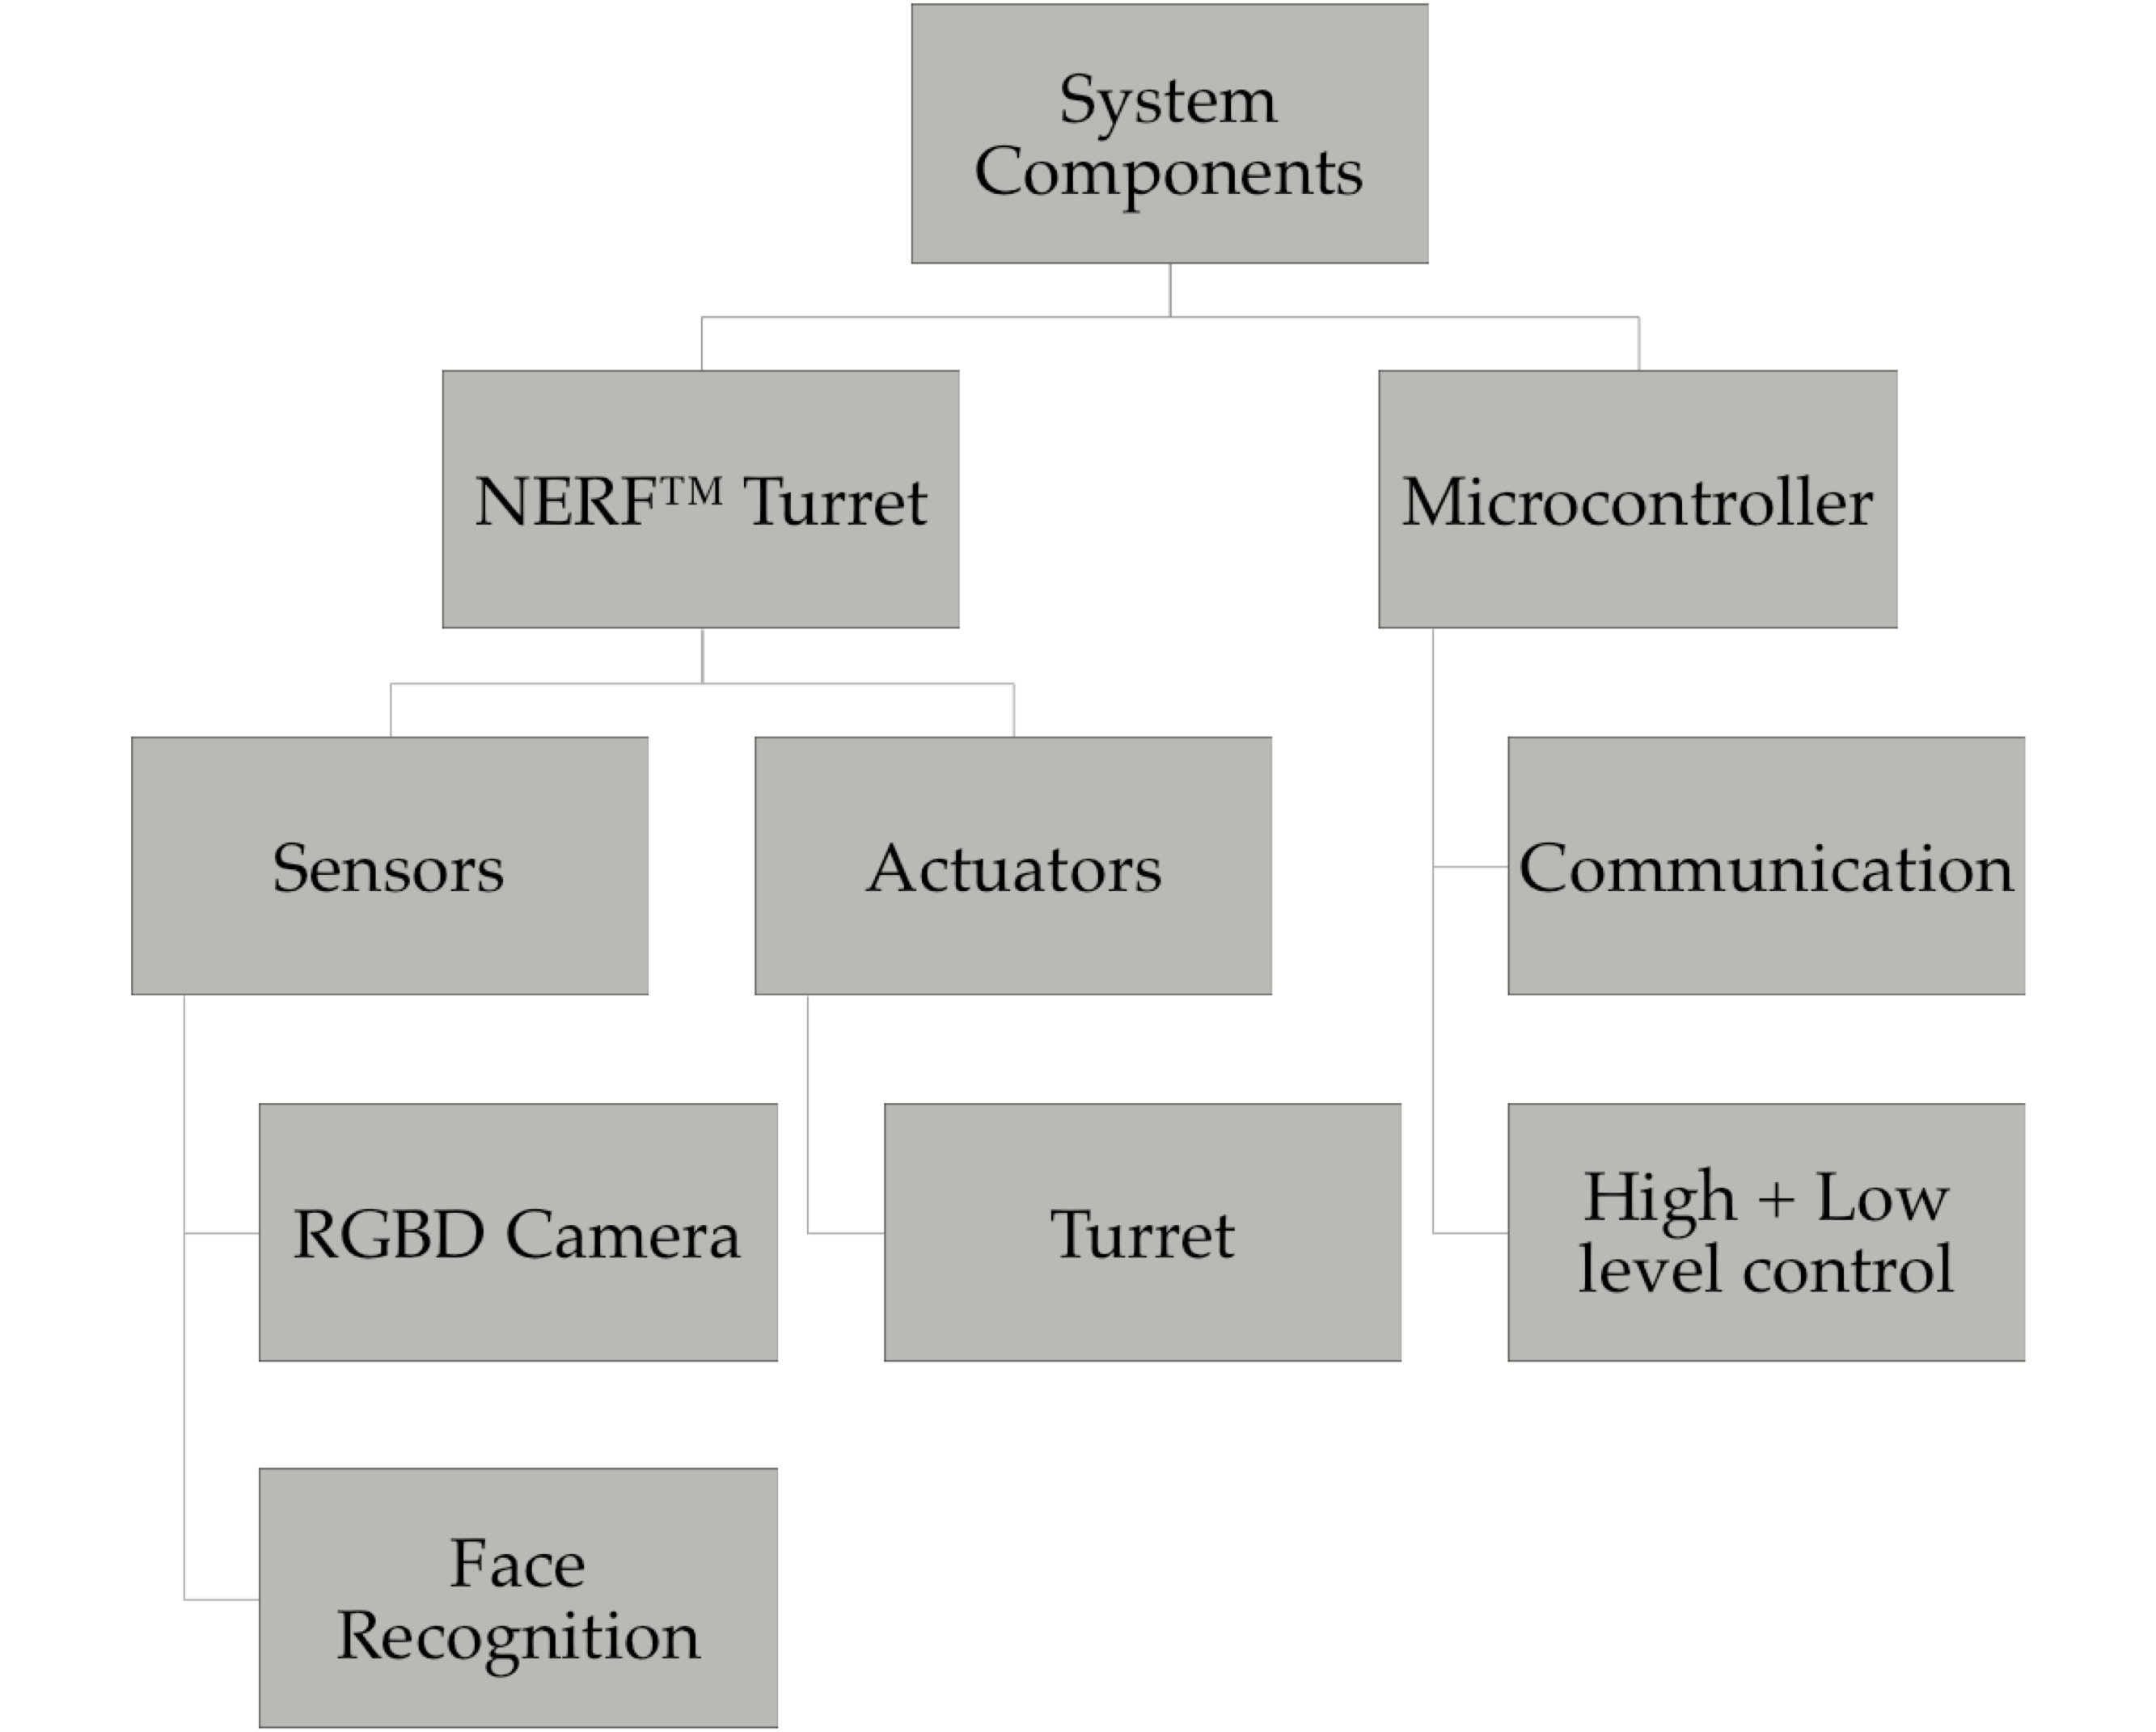
\includegraphics[width=0.80\linewidth]{components.png}
    \caption{System components hierarchy}
    \label{fig:components}
\end{figure}

In general, the system is divided into two overarching components: (1) the NERF Turret and (2) the Microcontroller. Each component can be subdivided further as shown in the diagram. In general, the NERF Turret component is responsible for providing the actuators that control the rotating platform - a turntable made of bearings, motors, and a winch -, an electronically triggered NERF gun mounted on the platform, and the RGBD camera sensor that performs the face recognition. On the other hand, the microcontroller component is responsible for providing the controller api calls that appropriately handle the high and low level control of the system. The microcontroller is connected to the actuators via wired connections, and to the sensors using a WiFi connection via the Adafruit CC3000 chip.

\section{NERF Turret Hardware}

The descriptions we have for our hardware in the NERF turret are described below.

\begin{figure}[htbp]
    \centering
    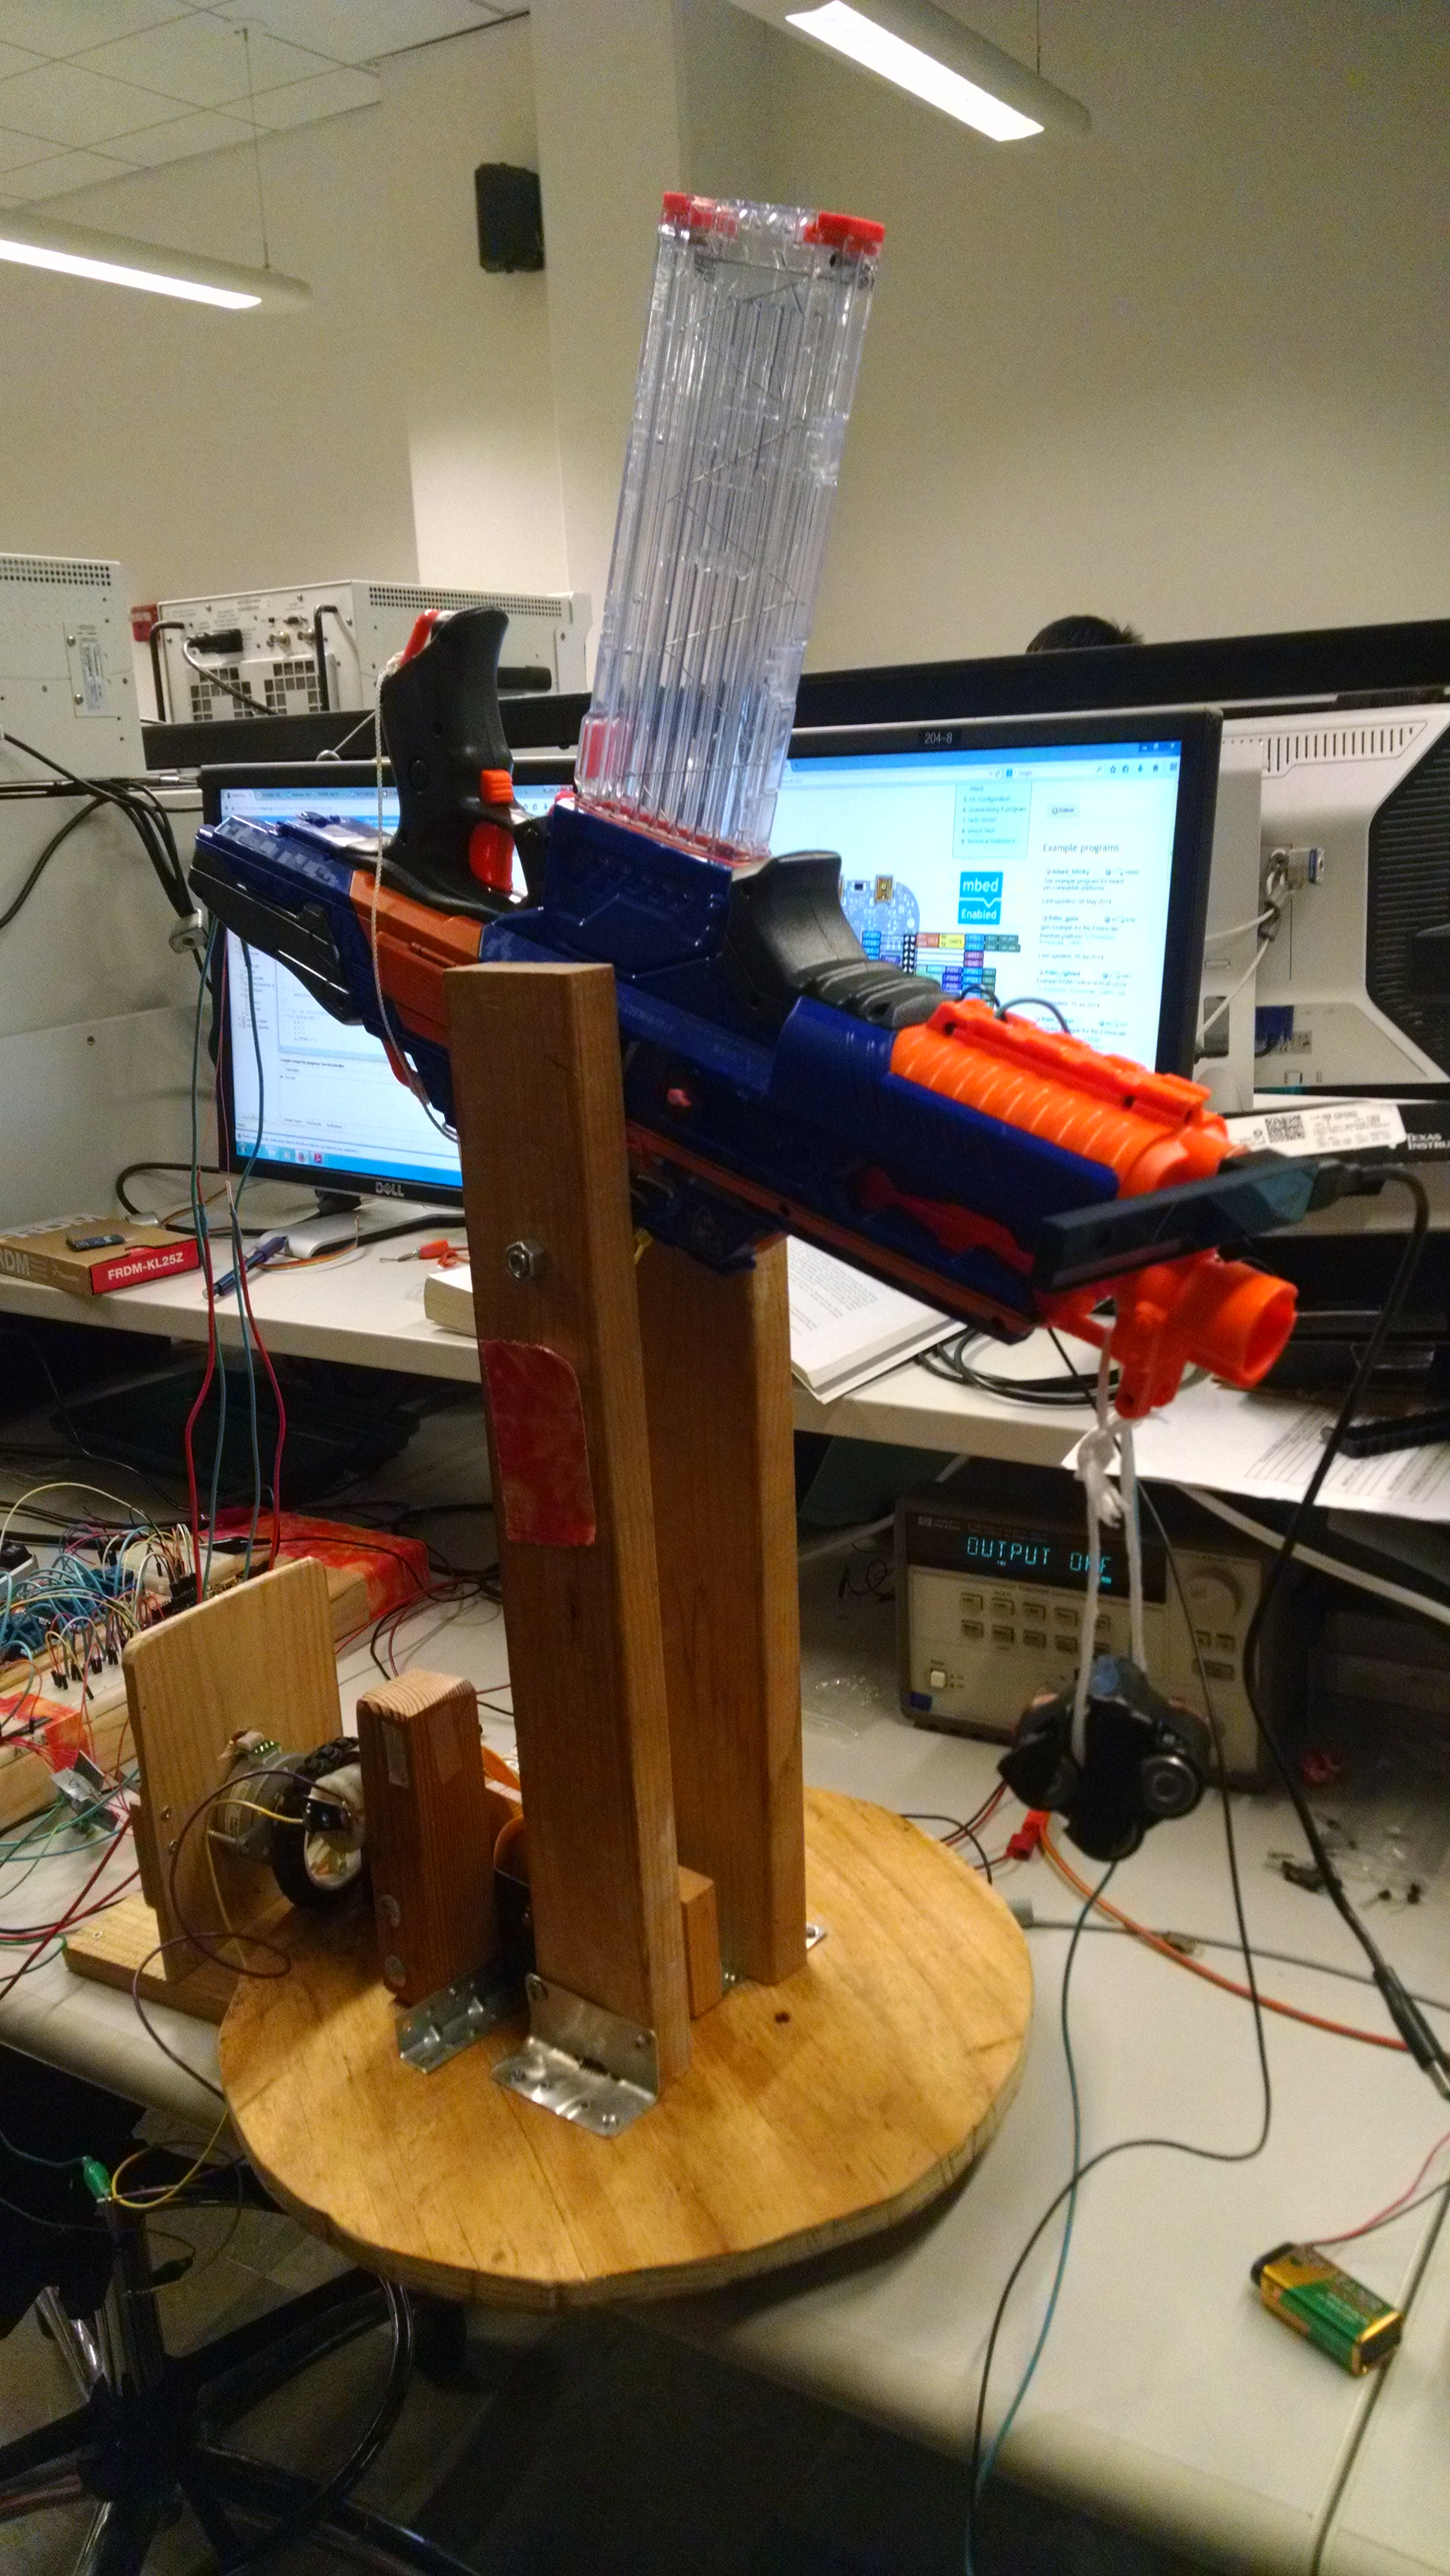
\includegraphics[width=0.60\linewidth]{fullturret.jpg}
    \caption{The actual NERF gun and turret.}
    \label{fig:fullturret}
\end{figure}

\subsection{NERF Gun}

\begin{figure}[htbp]
    \centering
    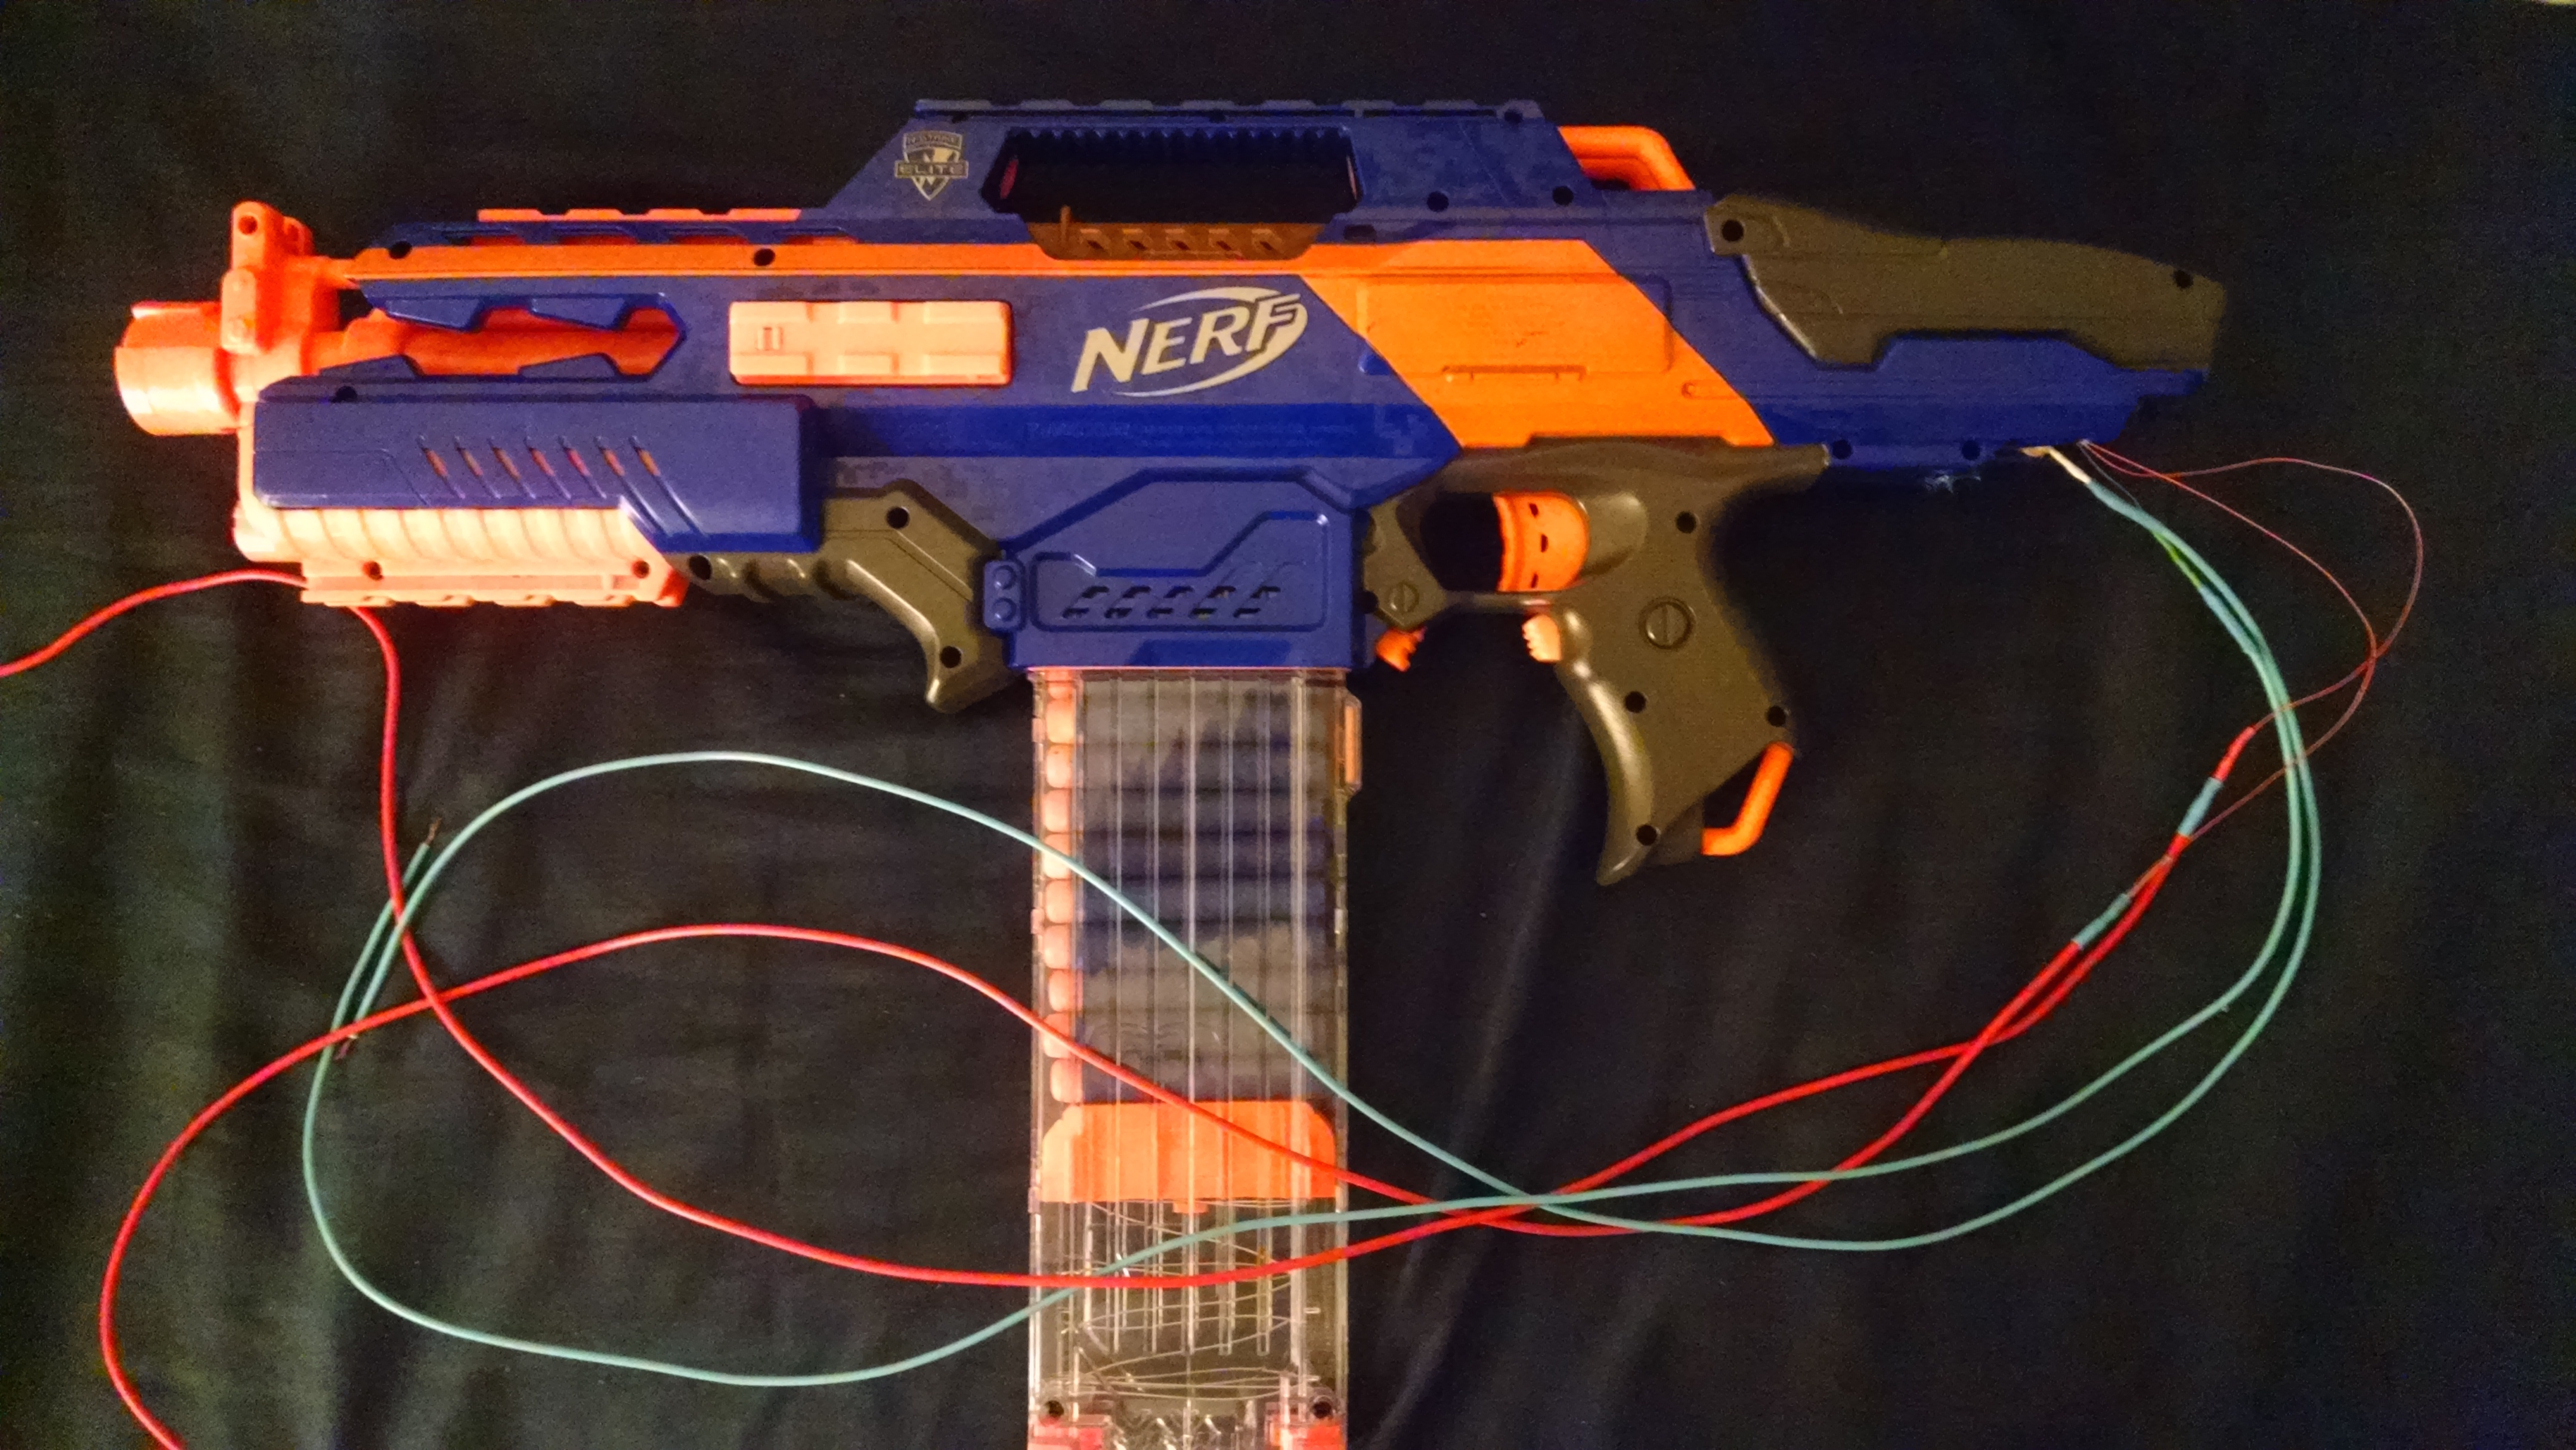
\includegraphics[width=0.80\linewidth]{gun.jpg}
    \caption{The CS-18 that has been modified to allow external control.}
    \label{fig:gun}
\end{figure}

The NERF gun and the motors on the turret are the actuators in our system. We selected the CS-18, which was chosen since it was not only relatively lightweight, but also entirely electronically controlled which allowed us to swap out the switches of the firing mechanism. Figure~\ref{fig:gun} below shows the result of disassembling the gun to allow electronic firing.

Currently, we have disassembled the NERF gun and reverse-engineered it to the point where we can electronically trigger it to fire a NERF dart. In addition, we have obtained two relays to replace the trigger switches in the gun in order to connect it to the microcontroller. Relays are used since they are more easily controlled via a GPIO pin on the microcontroller.


\subsection{Turret Motors}

\begin{figure}[htbp]
    \centering
    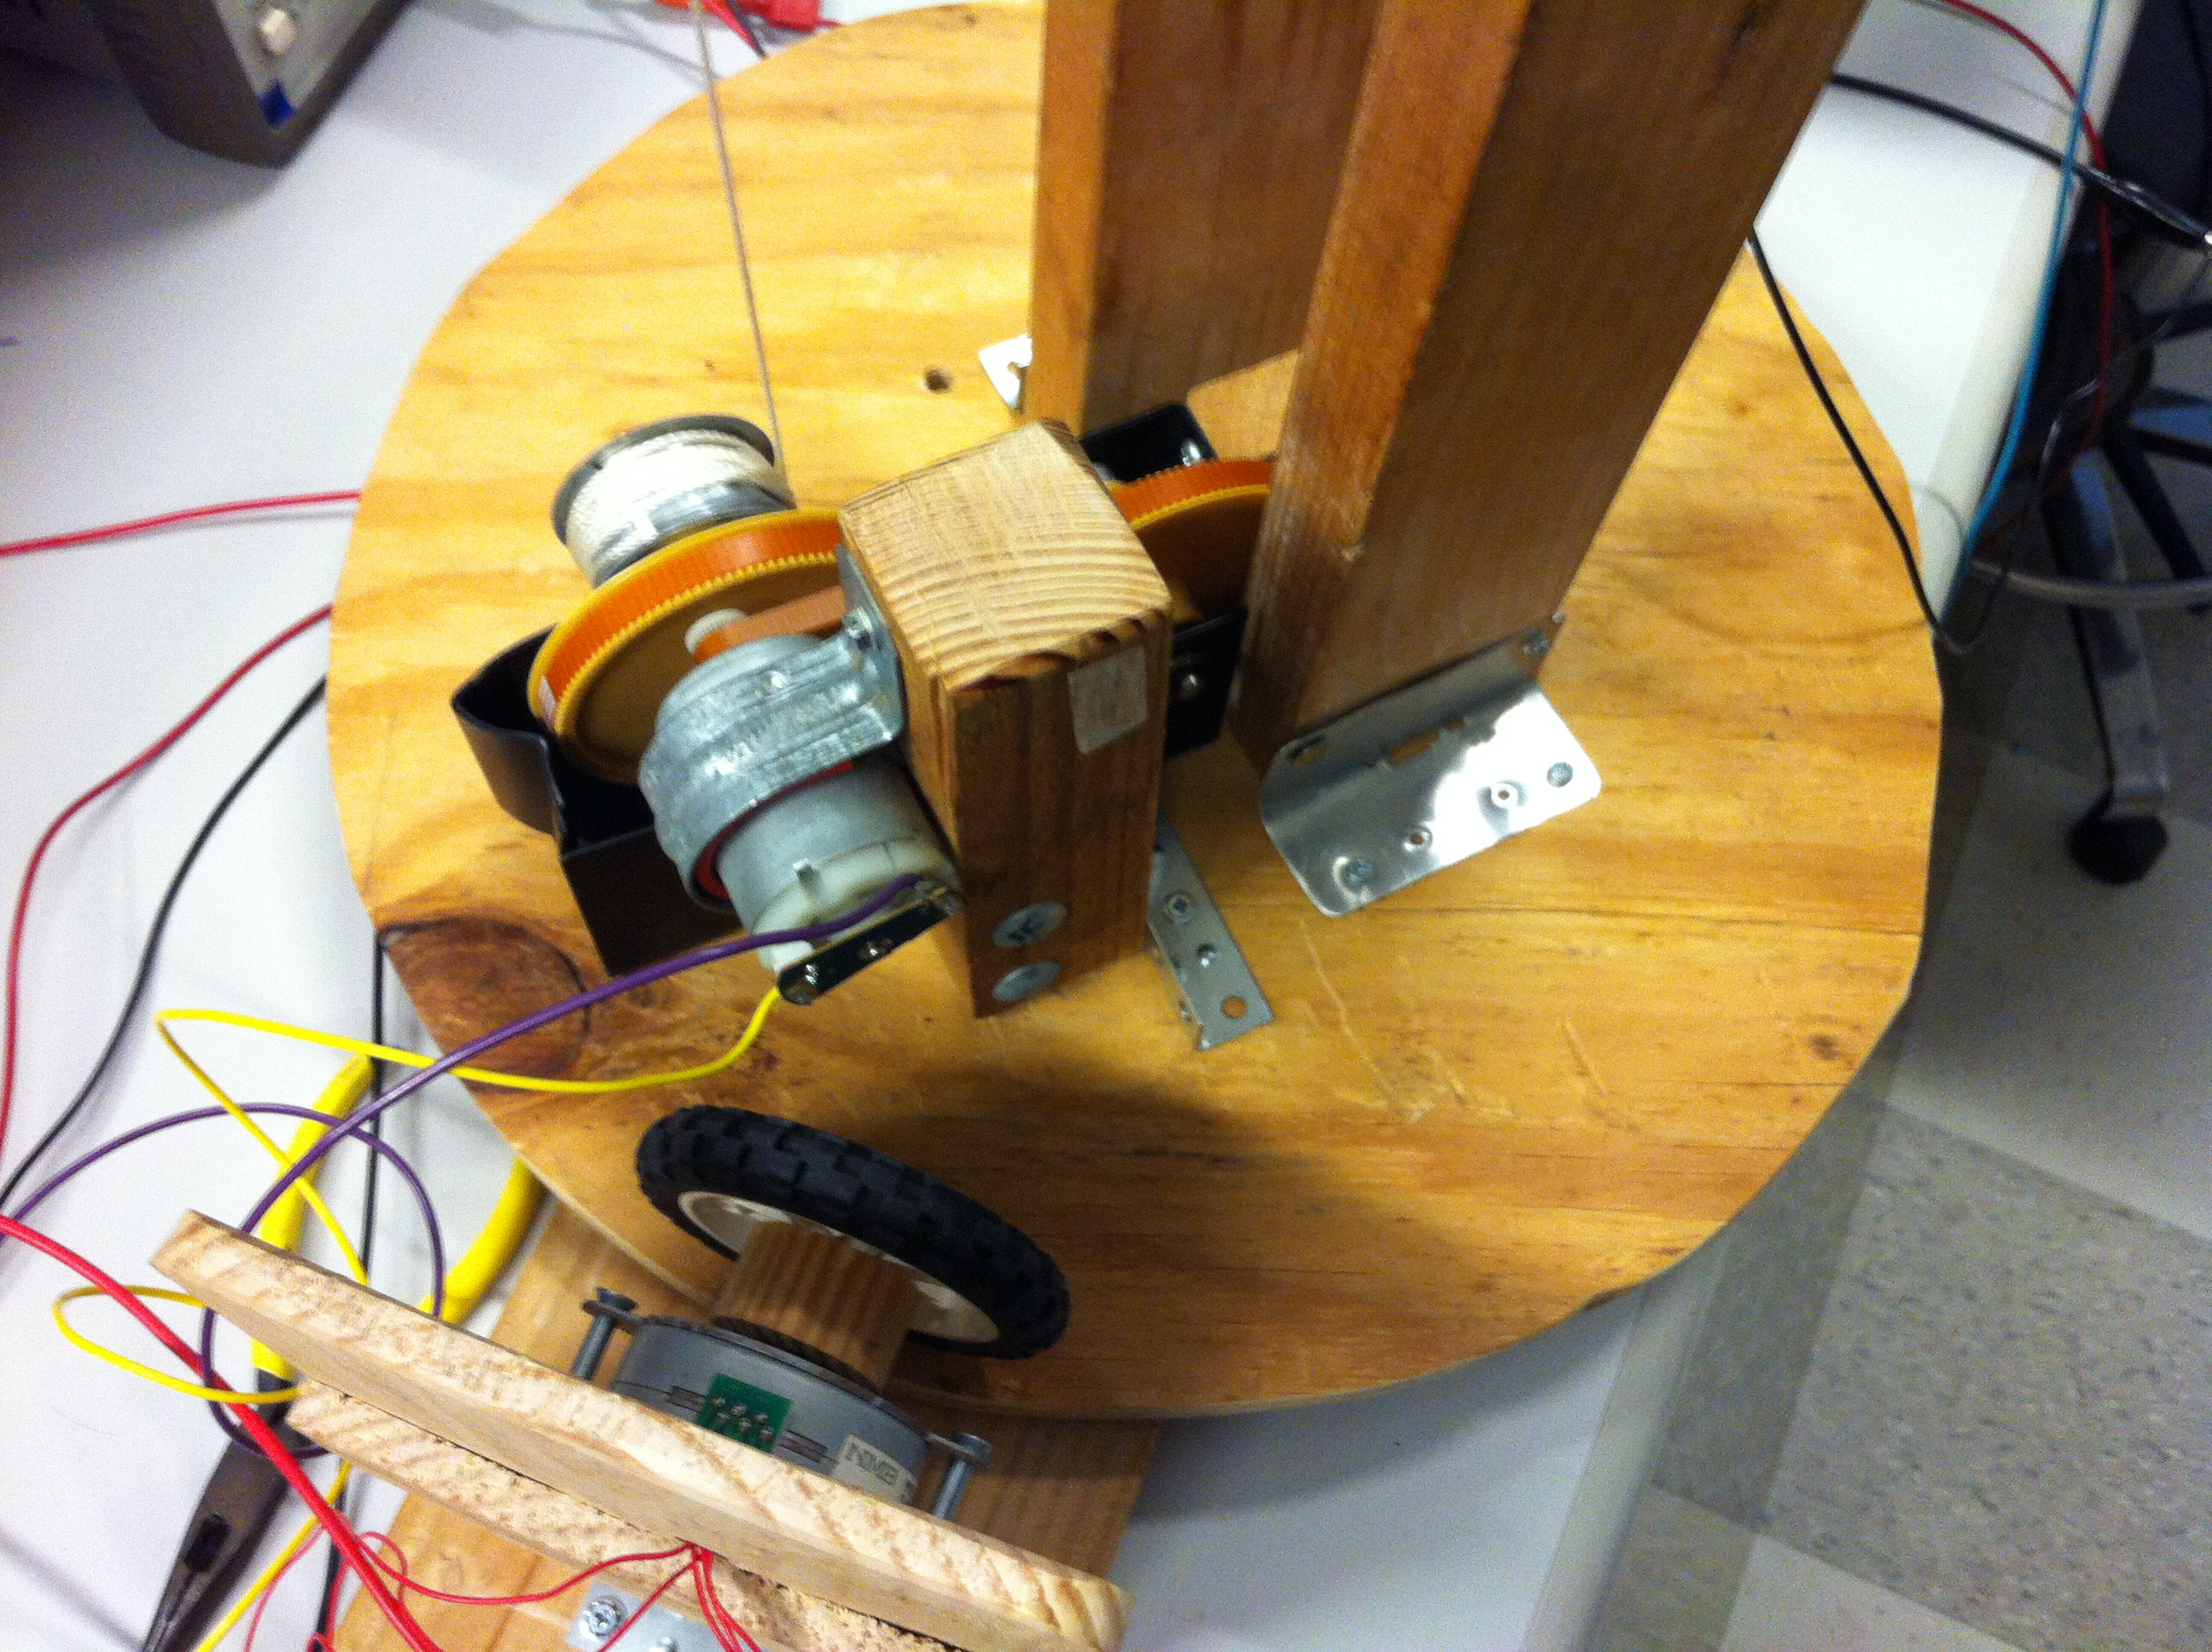
\includegraphics[width=0.80\linewidth]{motors.jpg}
    \caption{The turret for the NERF gun along with the two driving motors.}
    \label{fig:motor}
\end{figure}

We used pair of motors were used to control the turret; one for vertical motion, and one for horizontal.

Our turret is mounted on a turntable, and it is spinning this turntable that allows our NERF gun to rotate side to side. To control the turntable, we went with a stepper motor mounted with a wheel that lies on the rim of the turntable. By driving this motor, our wheel pushes our turntable, causing it to spin and giving us away to move the NERF gun. We decided to use a stepper motor because we felt that the control it gave us made it ideal for this role. We did not need a lot of torque since our turntable spun quite easly, so we could get away with using the stepper motor. Additionally, the stepper lets us have precise control of how many degrees it turned each time we sent it a signal from our microcontroller, which allows us to precisely aim our NERF gun.

As for up and down motion, we ended up using a DC motor that through gearing, had a very high torque. Because we mounted our NERF gun on a pivot, we wanted a motor strong enough to be able to pull the gun up and down. Since the NERF gun has a decent weight to it, we needed a pretty high torque motor in order to be able to move the gun. The motor has a strong string that it can wind up that is tied to the back of the gun, allowing us to be able to aim the gun higher or lower.

\subsection{Electronics}

\begin{figure}[htbp]
    \centering
    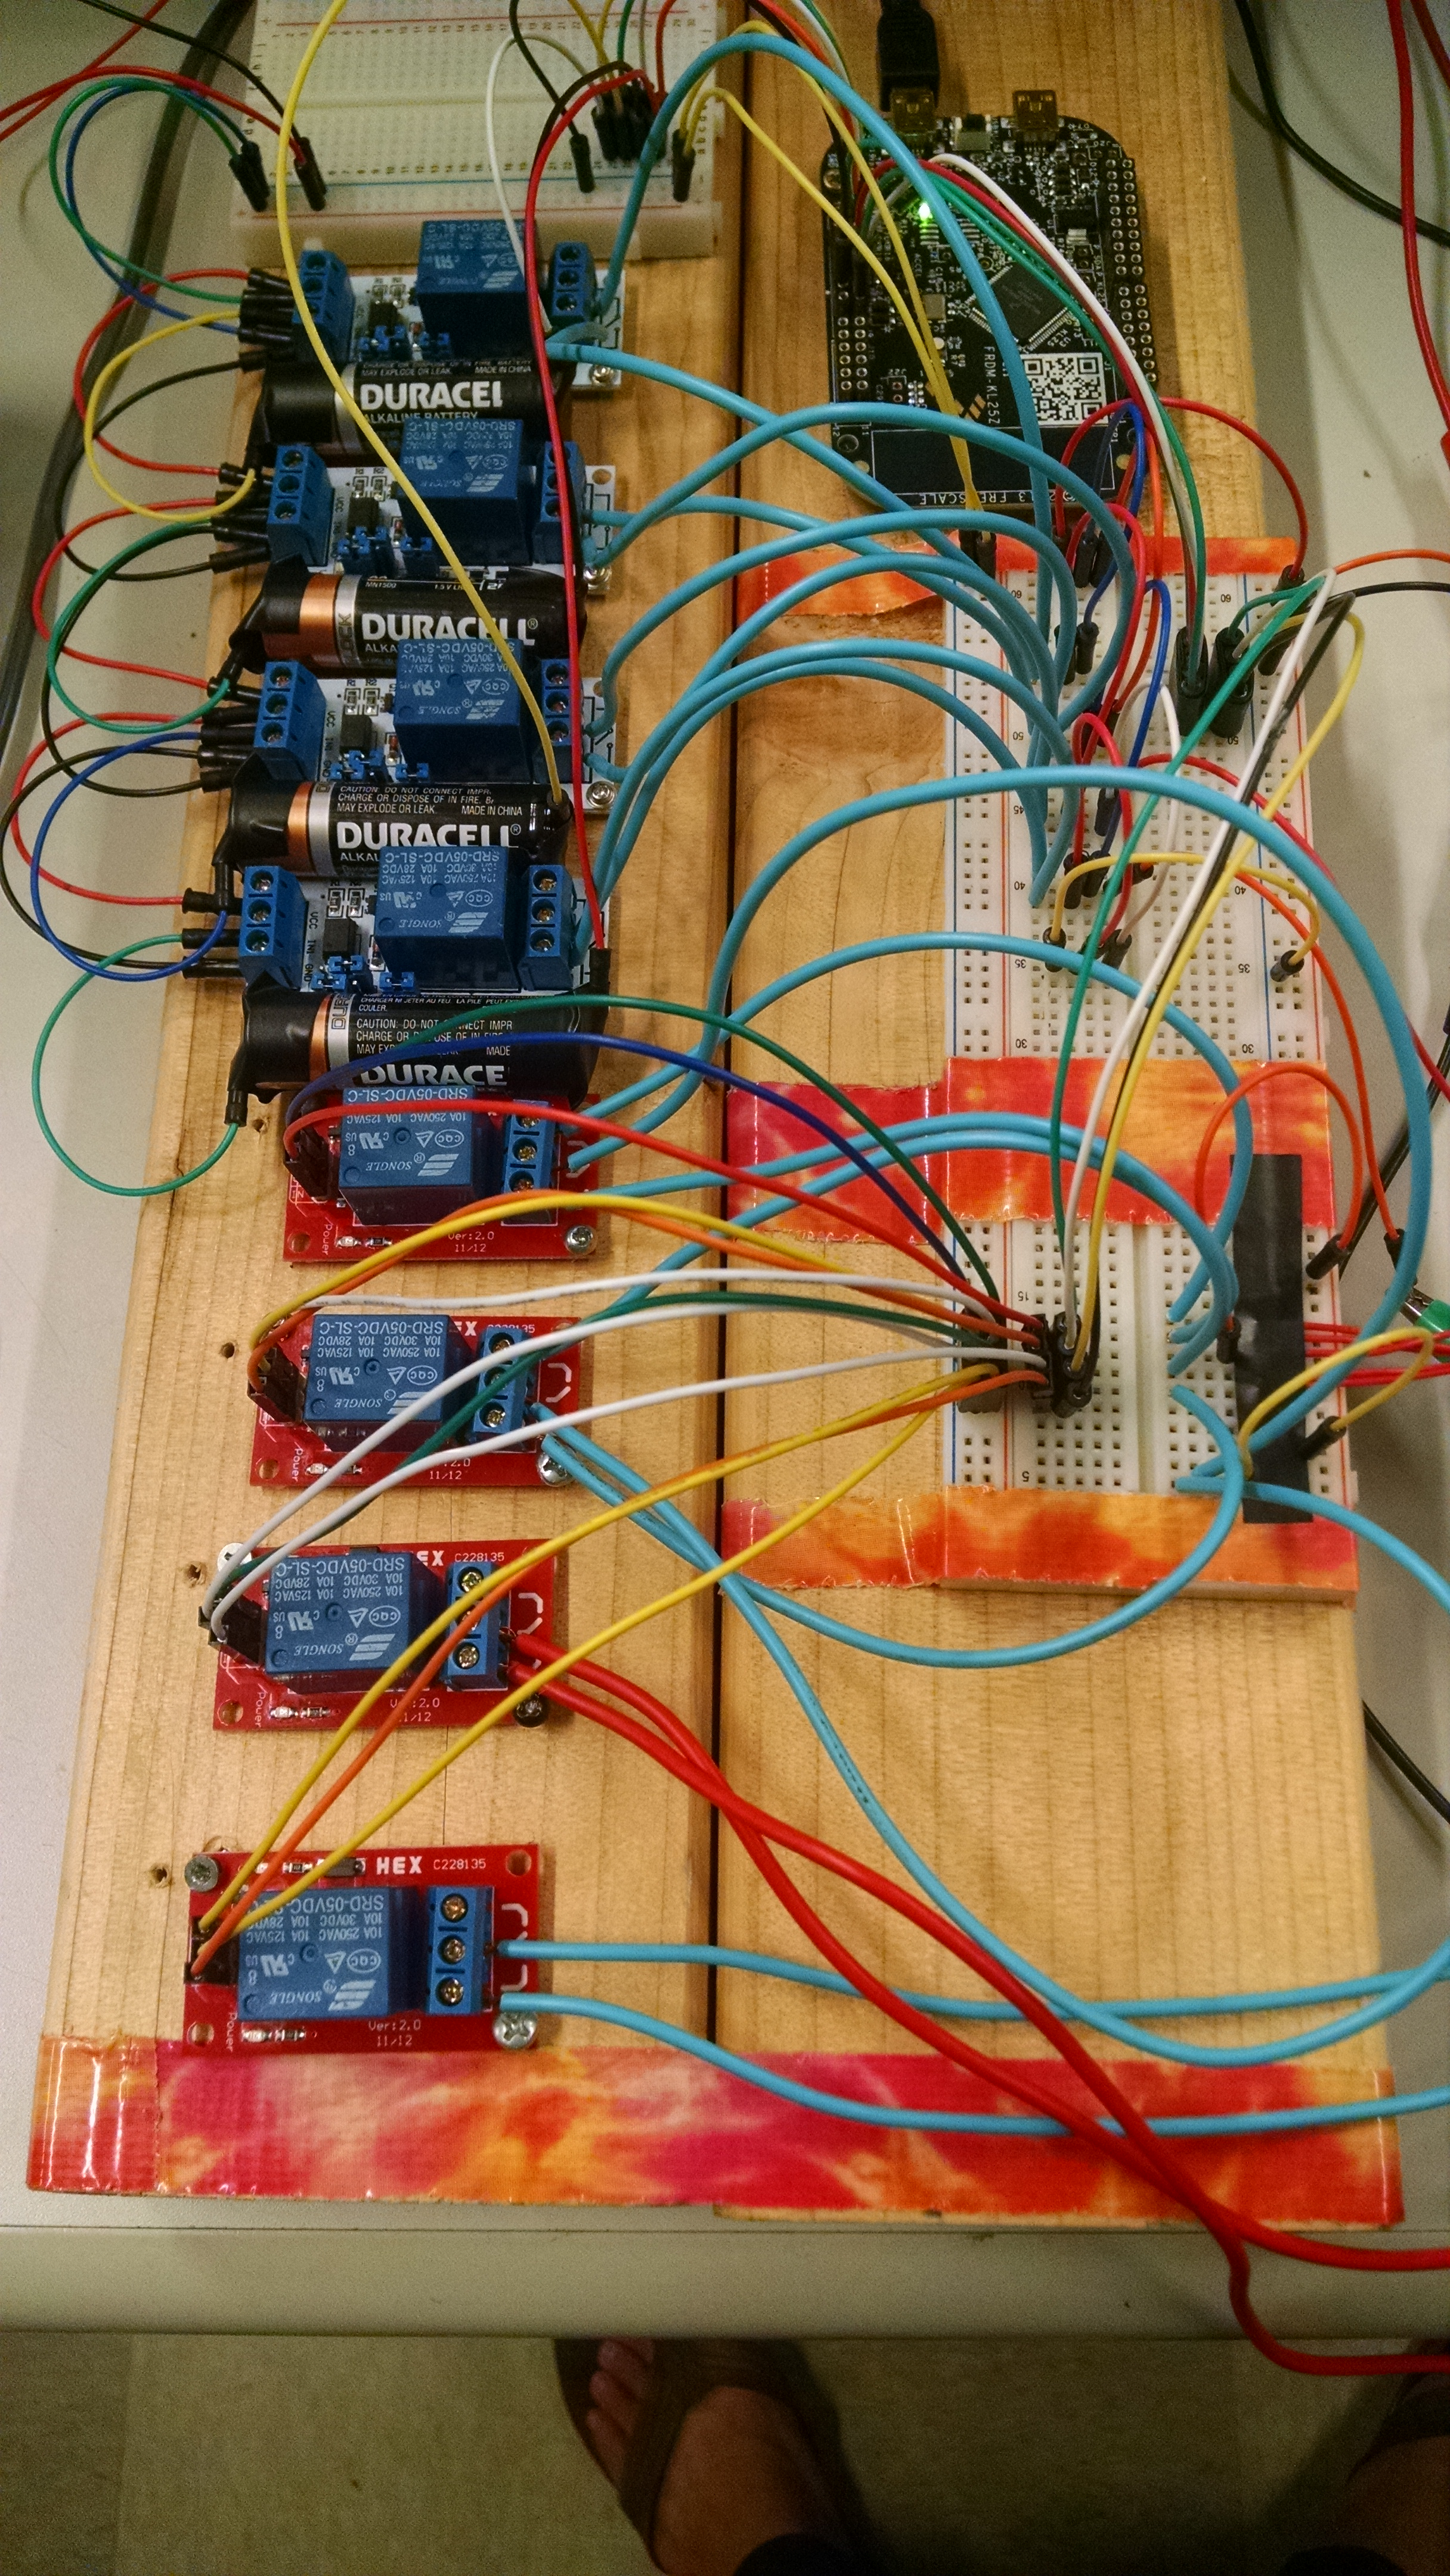
\includegraphics[width=0.60\linewidth]{electronics.jpg}
    \caption{The electronics mounted on a two by four. These are used mainly to control the turret firing and rotation.}
    \label{fig:electronics}
\end{figure}

In order to control our motors and the firing of the NERF gun, we relied on a series of relays that lets the MBED control when to send power to the various components of the NERF gun. We ended up using eight relays in total; four relays to control the DC motor, two relays to control the stepper motor, and two relays that dealt with the firing of the NERF gun.

We needed to create an H-Bridge in order to give our microcontroller the ability to switch the direction of the voltage driving the DC motor, allowing us to wind and unwind the string that controlled the up down motion of the NERF gun. An H-Bridge requires using four switches, hence four of our relays. The stepper motor could be controlled by senting voltages across the four wires that were attached to it, so we ended up using two of our relays here.

The final two relays were used to control the firing of the NERF gun. In order to fire, we had to have two things happen--the flywheels inside the gun had to be spinning, and the plunger had to push the NERF bullet into the flywheels. Both of these events could be done by connecting a pair of wires inside the gun for each functionality, so we had our two relays each control one of these functionalities.

\section{Camera and Controller}

\subsection{RGBD Camera, Face Recognition, and Server}

\begin{figure}[htbp]
    \centering
    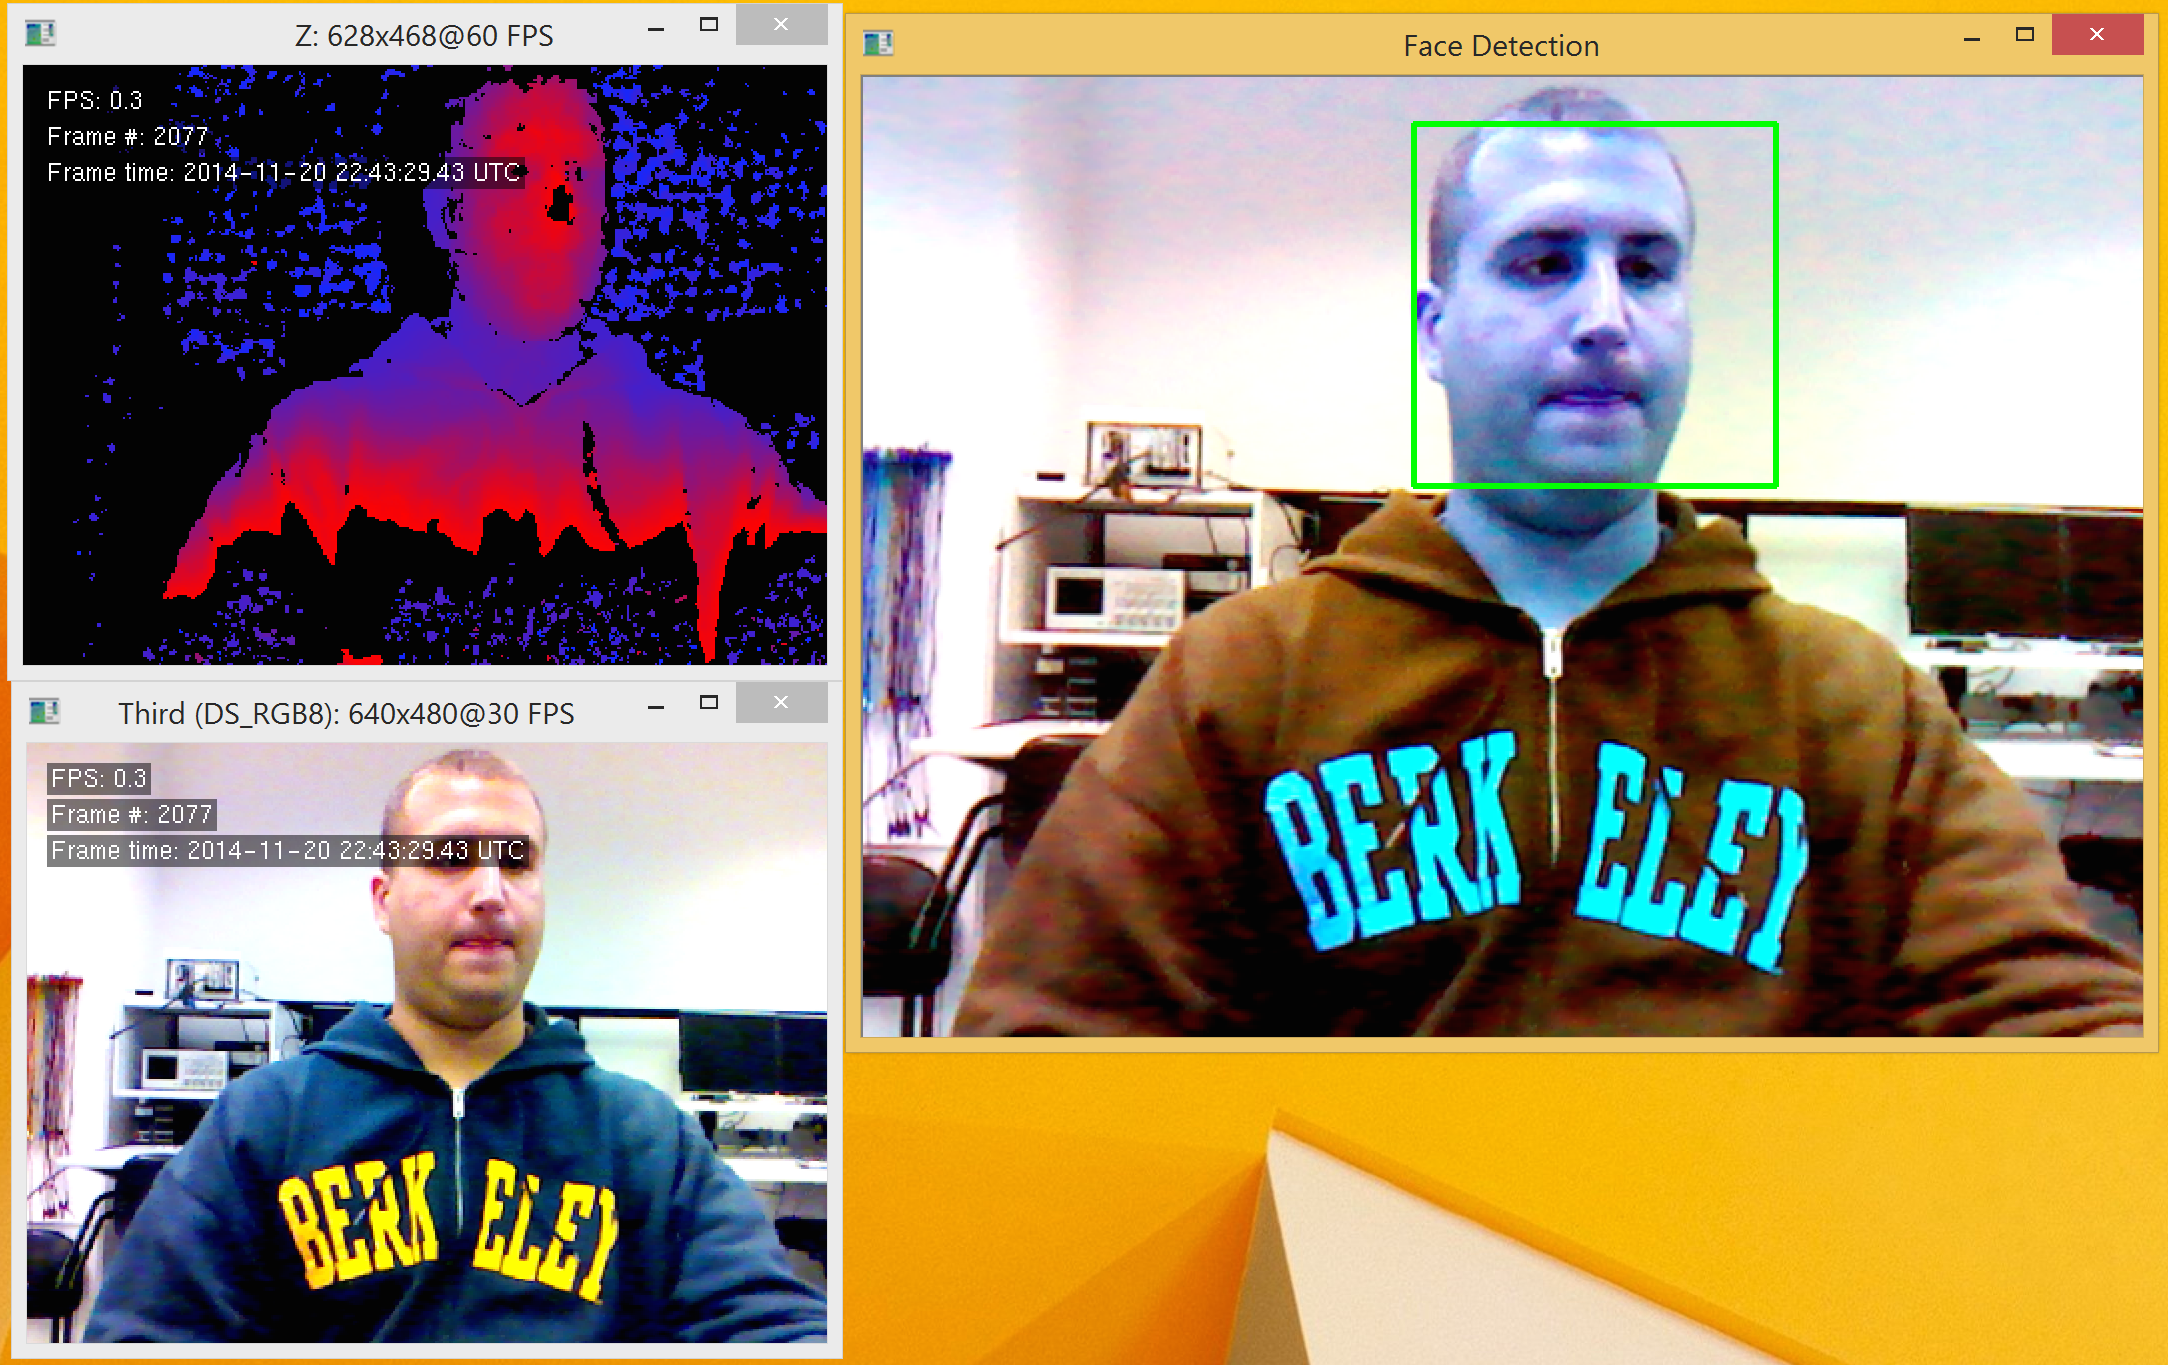
\includegraphics[width=0.85\linewidth]{face_detection.png}
    \caption{Going counter-clockwise  from the top right - Depth Map, RGB Image, and Face Detection}
    \label{fig:face}
\end{figure}

We have decided to use an Intel RealSense 3D Camera to handle face recognition. This camera was chosen since it has a small form factor and provides RGBD information at 30 frames per second. The RGB information is important in order to perform face recognition, and the depth information will be useful to allow the NERF gun to properly target the face once it is detected.

A limitation of this camera is that it must be connected to a Windows 8 computer via USB3, but it only came with a short cable. To get around this limitation, we ordered a 2 meter USB3 extension cable.

On the software side, we have C++ code that reads from the camera and uses OpenCV to detect faces. Figure~\ref{fig:face} shows a demo of this behavior. Once the code figures out where the face is, it sends a POST request containing the x and y coordinates of the face on the camera picture, the depth of the face, and a timestamp. The POST request is send to a node.js server running on Heroku, which our microcontroller can then pull these readings from.

\subsection{Controller}

\begin{figure}[htbp]
    \centering
    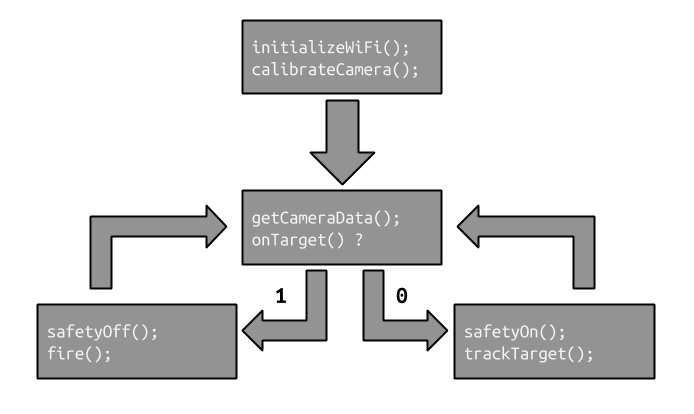
\includegraphics[width=1.0\linewidth]{controller_algo.png}
    \caption{Control flow graph of the turret controller}
    \label{fig:code}
\end{figure}

Finally, we have our MBED, which we are using to drive the actual aiming and firing of the NERF gun. In order to determine where to point the gun and when to actually shoot, we are relying on the measurements that are stored on our node.js server. To get these, we have decided to use WiFi for our connection scheme. While WiFi might not be the optimal choice if we wanted to track and shoot the target as fast as possible, we found it was the quickest way for us to satisfy our requirements. We used the Adafruit CC3000 chip in order to achieve this. Our MBED would send a GET request to the node.js server, which would return the coordinates of the target, which we would then use to aim and fire the gun.

Figure~\ref{fig:code} shows a high level view of the software ran on the MBED to drive the robot. In the very beginning of the controller program, various initialization are performed before the robot starts operating: web connection is set up for getting camera data and camera is calibrated to ensure accuracy. Next, the robot gets the camera data and checks if it is aiming at the target with some tolerance, if yes, the robot fires the NERF gun, if no, it adjusts its orientation to try to track the target. Afterward, the robot gets the camera data from the node.js server and checks if it is aiming at the target, and the cycle repeats ad infinitum.

\section{Real Time Networks and Timing}

\begin{figure}[htbp]
    \centering
    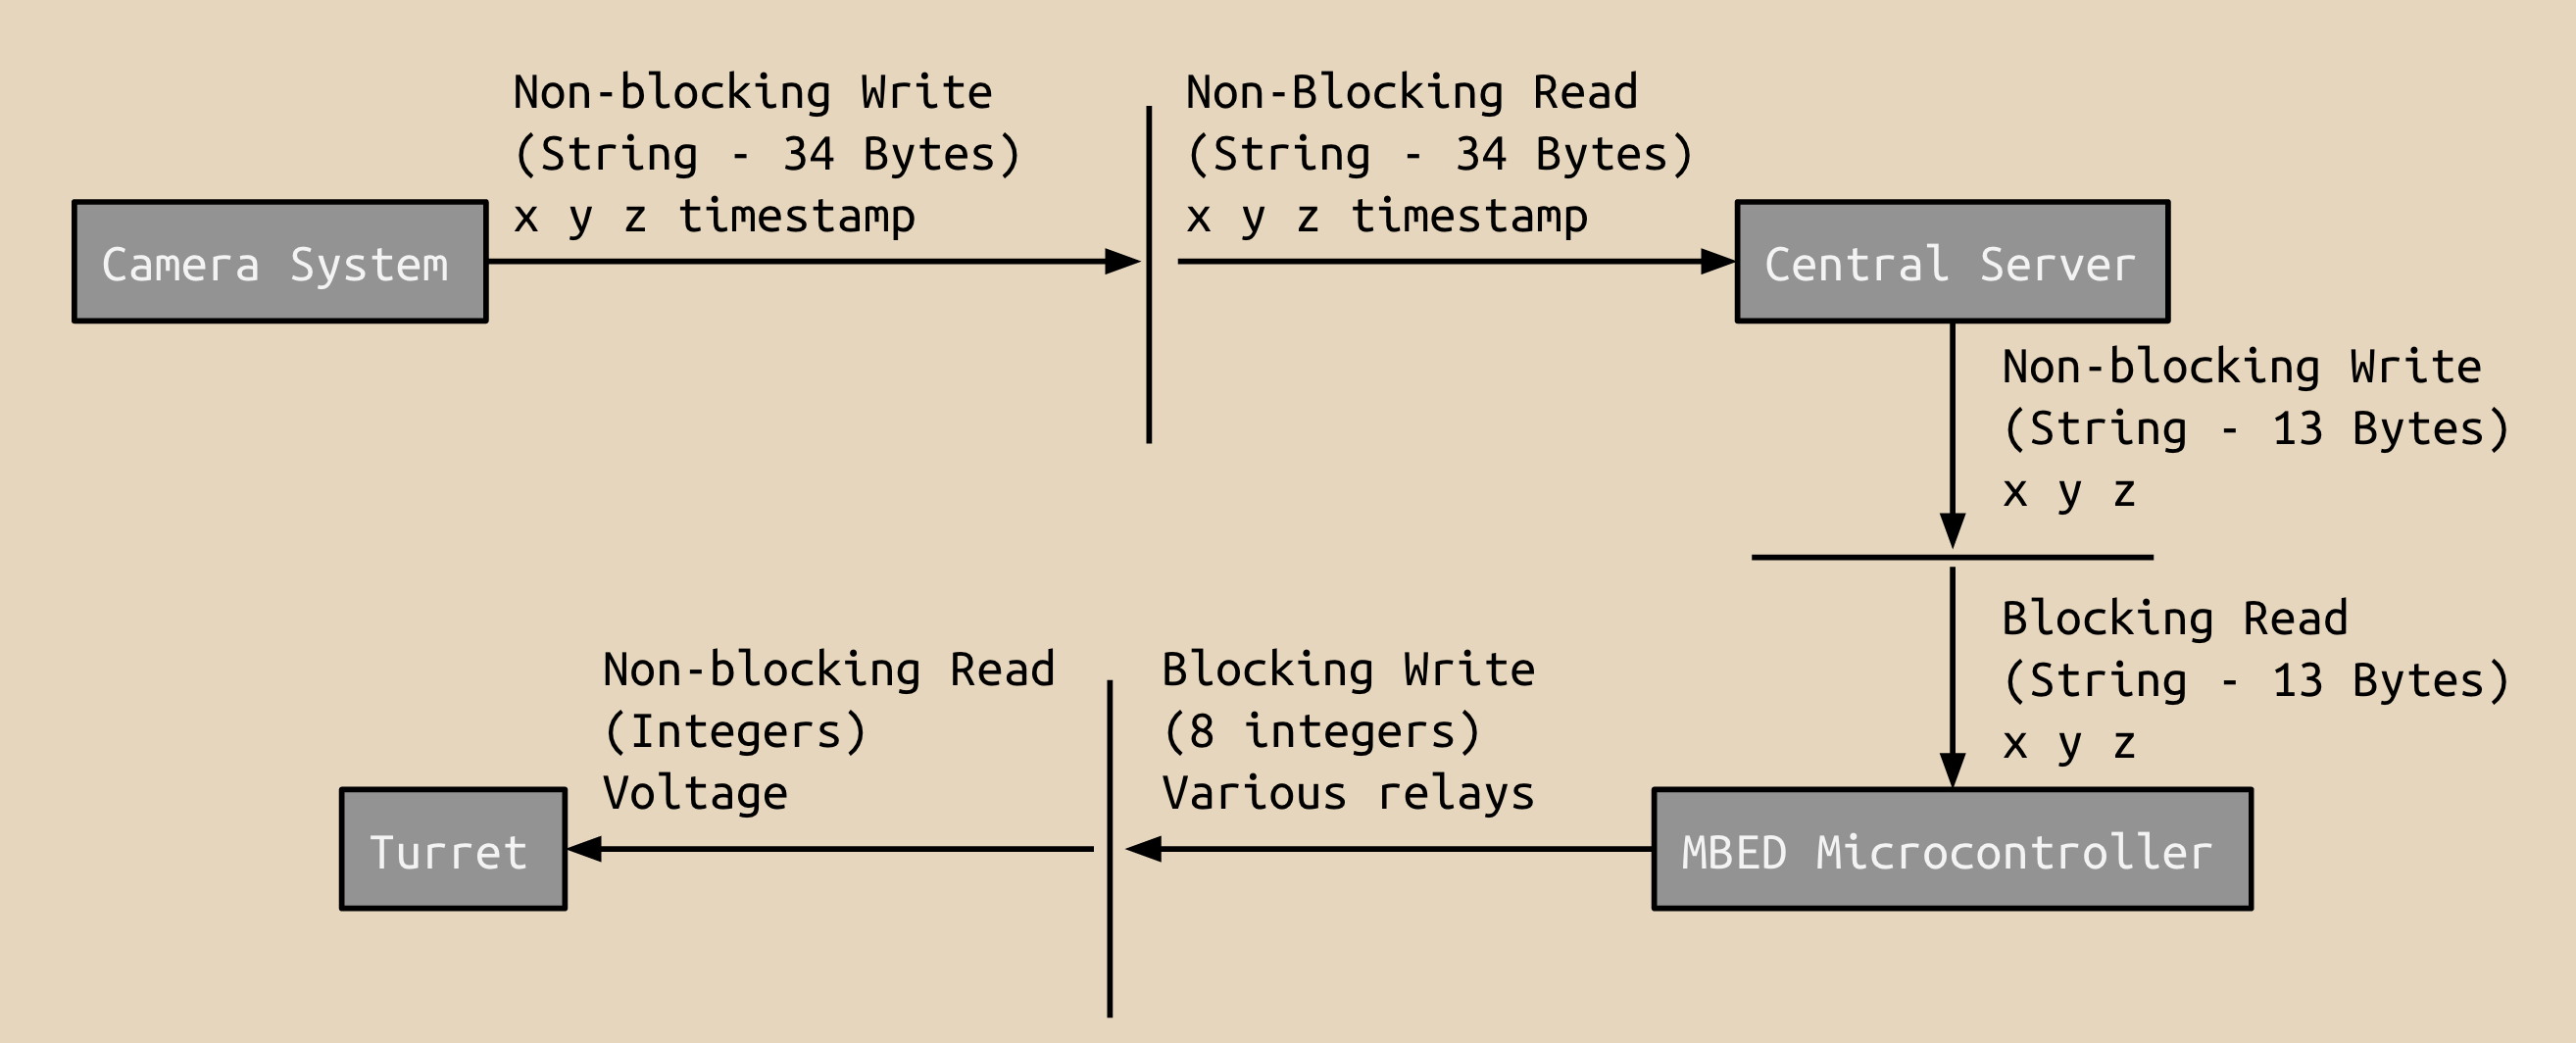
\includegraphics[width=0.99\linewidth]{network.png}
    \caption{Networking interactions between the camera, server, and MBED}
    \label{fig:network}
\end{figure}

A large part of getting our system to work involved getting our modules to communicate with each other in real time. To do this, we had to design our communication network to be able to control the NERF gun within a reasonable window to allow it to actually hit people.

Our communication network consists of three main entities talking to one another--the camera, the central sever, and the MBED. The interactions between these systems can be seen in the diagram. Most of the inter system communication was done using WiFi--we found that it was the easiest solution for us to implement that still gave us performance good enough to meet our criteria. We found that the latency of the WiFi components were roughly 100 milliseconds, which we found was perfectly reasonable for our system. Also, we made sure that we made as much of the communication non blocking as possible, so that our reads and writes would not hang if we could help it.

We ended up able to get our getting the communication between the camera and server to be a non blocking write to optimize our network, while our MBED pulls from the server in a non blocking read, which follows the observer design patter (camera writes, MBED observers, so we don't get any conflicts). The only blocking communication we had was the actual control of the turret with a blocking write to control the MBED.



\section{Realtime Behavior}
There were a few techniques that we used in the class to try to get as best performance out of our system as possible. We programmed in hysteresis into our system for aiming the NERF gun, so that we wouldn't have this wobbling back and forth cycling effect where our system can't reach the exact position that it wants to. We also had a delta for our firing window in order to give us some cushion about when we could shoot, which also helped our system achieve it's target more quickly.

\section{Future Goals}

While we did manage to meet our requirements with the robot we presented, there are a few areas of improvements that we can work on if we were to continuing developing our project.

On the hardware side of things, we found that our wiring and packaging of all the compenents was not done very well--the compenents have a very large footprint, with wires spanning all over the place. We sometimes found that our wiring, because of the packaging, was limiting how much our turret could rotate. Additionally, the wiring schematic was not particuarily planned out to minimize the footprint initially, so a smarter packaging system would improve our system greatly.

Additionally, we want to look at speeding up our target aquisition and firing so would could perhaps track a moving target. With our current motor and WiFi setup, we can find and hit a static target pretty easily, but our system does not move fast enough to track something moving. Ways to improve this would be to try a faster network protocol, such as using wired connection instead of wireless, or optimizing our code in order to speed up facial recognition or controlling the movement of the robot. We could also modify our algorithm to make the turret move fast if our target is further away in order to lower the number of times we need to poll the camera.

%============================================================
% BIBLIOGRAPHY
%============================================================

\nocite{*}
\bibliographystyle{IEEEtran}
\bibliography{sources}

% that's all folks
\end{document}


